\chapter{Sequences}

\section{Lists and Containers}
\begin{itemize}
    \item List: a compound value (sequence of values)
    \item A method of combining data values satisfies the \emph{closure property} if the result of the combination can itself be combined using the same method
    \item i.e. Lists can contain lists as elements
    \medskip
	\begin{figure}[H]
	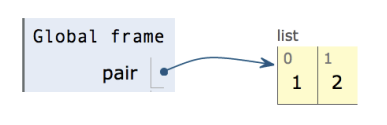
\includegraphics[width=0.5\linewidth]{figures/env_diagram_list.png}
	\caption{List Format in Environment Diagrams}
	\end{figure}
\end{itemize}

\section{For Statements}
\begin{itemize}
    \item Anatomy: for <name> in <expression>:
    \item Execution:
    \begin{enumerate}
        \item evaluate <expression>, which must yield an iterable value (sequence)
        \item For each element in that sequence in order: 
        \begin{enumerate}
            \item Bind <name> to that element in the current frame
            \item Execute the suite
        \end{enumerate}
    \end{enumerate}
\end{itemize}

\section{Ranges}
\begin{itemize}
    \item Range: a sequence of consecutive integers
    \item Starting value (inclusive) to enging value (exclusive)
    \item Length: ending value - starting value
\end{itemize}

\section{List Comprehensions}
\begin{itemize}
    \item Combined expression that evaluates to a list
    \item Anatomy: [<map exp> for <name> in <iter exp> if <filter exp>]
    \item Anatomy without filter: [<map exp> for <name> in <iter exp>]
    \item For each element in <iter exp> if <filter exp> is True, then add <map exp>
\end{itemize}

\section{Slicing}
\begin{itemize}
    \item Slicing a list creates new values, does not reference original list values
    \item Anatomy: <new list name> = <list name>[<start index>:<end index>]
    \item If no explicit start or end index, the beginning or end of the list is used
    \item Start index is inclusive, end index is exclusive
\end{itemize}

\section{Aggregation}
\begin{itemize}
    \item Built-in functions:
    \item sum(iterable[, start]) -> value
    \item Returns the sum of an iterable + start (default start value is 0)
    \item max(iterable[, key=func]) -> value
    \item Returns the largest item in the iterable, based on key function (default is no function)
    \item all(iterable) -> value
    \item Returns True if all values in the iterable are True (including empty iterable), False otherwise
\end{itemize}

\section{Strings}
\begin{itemize}
    \item String literabls are surrounded with single or double quotes
    \item A backslash "\textbackslash" escapes the next character
    \item Line feed character "\textbackslash n" represents a new line
\end{itemize}

\section{Dictionaries}
\begin{itemize}
    \item Dictionary: a collection of key-value pairs
    \item Keys must be unique within the same dictionary
    \item Keys cannot be a list or dictionary
    \item Dictionary comprehension: \{<key exp>: <value exp> for <name> in <iter exp> if <filter exp>\}
\end{itemize}